%Removing overlays from a beamer presentation is easily done within the preamble,
%by adding the handout option
%\documentclass[handout,xcolor=pdftex,dvipsnames,table,notheorems]{beamer} 
%\usepackage{pgfpages}
%\pgfpagesuselayout{4 on 1}[a4paper,border shrink=5mm,landscape]

\documentclass[notheorems,hyperref={bookmarks=true}]{beamer}
\usepackage[framesassubsections]{beamerprosper}
\hypersetup{pdfpagemode=FullScreen}
\usepackage[utf8]{vietnam}
%\usepackage[tcvn]{vietnam}
\usepackage[english]{babel}
\usepackage{ulem} %for underlying+
\usepackage{pifont} %for creating dingautolist
\usepackage[mathscr]{eucal}
\usepackage{amsmath, amsthm, amssymb,amsxtra,latexsym,amscd,graphics,graphpap}
\usepackage{indentfirst}
\usepackage{rotating}
\usepackage{graphicx}
\usepackage{amsbsy}
\usepackage{epsfig}
\usepackage{natbib}
%\usepackage{pst-plot}
%\usepackage{msc}
%\usepackage{musixtex}
\usepackage{pdfpages}
\usepackage{multicol}
\usepackage{hyperref}
\usepackage{subfigure}
\usepackage{multimedia}
\usepackage{boxedminipage}
\usepackage{tikz}
\usepackage{nicefrac}
\setbeamertemplate{theorems}[numbered] % Đánh số định lý.

%\usetheme{Warsaw}
%\usetheme{Berlin}
%\usetheme{Madrid} 
%\usetheme{boadilla} 
%\usetheme{CambridgeUS} 
%\usetheme{Goettingen}
%\usetheme{Boadilla} % puts title, section, etc on top
%\usetheme{PaloAlto} % top and left bar.  left bar has outline
%\usetheme{Berkeley} % similar to Palo Alto
%\usetheme{Hannover}  % left bar with outline
%\usetheme{AnnArbor}
%\usetheme{Pittsburgh}
%\usetheme{Antibes}
%\usetheme{JuanLesPins}
%\usetheme{Montpellier}
%\usetheme{Szeged}
\usetheme{Copenhagen}
\usecolortheme{rose} 
\usefonttheme[onlylarge]{structurebold}
\usefonttheme{professionalfonts}
%\useoutertheme{smoothbars}
\usepackage{array}
\setbeamercolor{title}{fg=red!80!black,bg=blue!20!white}
\setbeamertemplate{section in head/foot shaded}[default][20]
\setbeamertemplate{subsection in head/foot shaded}[default][20]
\setbeamertemplate{navigation symbols}{}
\setbeamertemplate{blocks}[rounded][shadow=true]
\setbeamerfont{small}{size=\small}
\setbeamerfont{footnote}{size=\footnotesize}
\setbeamerfont{script}{size=\scriptsize}
\setbeamerfont{tiny}{size=\tiny}

\providecommand{\R}{\mathbb{R}}
\providecommand{\Mat}{\textsc{MatLab }}
\providecommand{\lr}[1]{\left( #1 \right)} 
\providecommand{\Lr}[1]{\left[ #1 \right]}
\providecommand{\LR}[1]{\left\{ #1 \right\}} 
\providecommand{\abs}[1]{\left\vert #1 \right\vert} 
\providecommand{\norm}[1]{\left\Vert #1 \right\Vert} 
\providecommand{\ov}[1]{\overline {#1}} 
\providecommand{\e}{\varepsilon} 
\DeclareMathSymbol{\INT}{\mathop}{largesymbols}{"5A} 
\renewcommand{\int}{\INT} 
\renewcommand{\iint}{\mathop{\int\!\!\!\!\!\int}}
\renewcommand{\iiint}{\mathop{\int\!\!\!\!\!\int\!\!\!\!\!\int}}
\DeclareMathOperator{\sinc}{sinc}

\theoremstyle{plain}
%\theorembodyfont{\slshape}
\newtheorem{definition}{Định nghĩa}[section]
\newtheorem{proposition}{Mệnh đề}[section]
\newtheorem{theorem}{Định lý}[section]
\newtheorem{lemma}{Bổ đề}[section]
\newtheorem{corollary}{Hệ quả}[section]
\newtheorem{conjecture}{Dự đoán}[section]
\newtheorem{remark}{Chú ý}[section]
\newtheorem{example}{Ví dụ}
\newtheorem{problem}{Bài toán}[section]
\newtheorem{exercise}{Bài tập}

\renewcommand{\thedefinition}{\arabic{section}.\arabic{definition}}
\renewcommand{\thelemma}{\arabic{section}.\arabic{lemma}}
\renewcommand{\thetable}{\Roman{table}}
\renewcommand{\thetheorem}{\arabic{section}.\arabic{theorem}}
\renewcommand{\thecorollary}{\arabic{section}.\arabic{corollary}}
\renewcommand{\theequation}{\arabic{section}.\arabic{equation}} 
\renewcommand{\thefootnote}{(\arabic{footnote})}
\renewcommand{\theexample}{\arabic{example}}
\renewcommand{\theproblem}{\arabic{section}.\arabic{problem}}
\renewcommand{\theexercise}{\arabic{exercise}}
\mode<presentation>
\setbeamertemplate{navigation symbols}{} 
\numberwithin{equation}{section}
%\logo{\includegraphics[height=1cm]{logo.pdf}}
%\logo{%
%    \includegraphics[width=1cm,height=1cm,keepaspectratio]{logo.pdf}~%
%    \includegraphics[width=1cm,height=1cm,keepaspectratio]{logo.pdf}~%    
%}
\pgfdeclareimage[height=1cm]{fami-logo}{sami.png}
%\pgfdeclareimage[height=1.5cm]{hust-logo}{logo}
\logo{\pgfuseimage{fami-logo}}
%\setbeamertemplate{footline}{\raisebox{-2.2ex}{\pgfuseimage{hust-logo}}}


\usebackgroundtemplate{%
\tikz\node[opacity=0.15] {
\includegraphics[height=\paperheight,width=6 cm]{logi_Hust.png}};}


\begin{document}
\title[Tính Toán Song Song]
{TÍNH TOÁN SONG SONG\\HỆ THỐNG HỌC SÂU PHÂN TÁN \\[0.5 cm]}
\institute[SAMI-HUST]
{
	\Large Viện toán ứng dụng và tin học\\
	Đại học bách khoa Hà Nội\\[1.2 cm]
	
}
\author[Nguyễn Hữu Thuật (20185410)]{\large Sinh viên thực hiện: Nguyễn Hữu Thuật\\[0.5 cm]} 

\date{Tháng 08 năm 2021}
\logo{
\includegraphics[height=1.0 cm]{sami.png}}
%%===============
\begin{footnotesize}
\begin{frame}
	\frametitle{}
	\maketitle
\end{frame}

\AtBeginSection[] % Do nothing for \section*
{
	\begin{frame}<beamer>
		\frametitle{Nội dung}
		\tableofcontents[currentsection, currentsubsection]
	\end{frame}
}

\begin{frame}{Lý do chọn đề tài}
\begin{enumerate}[i.]
	\item Trí tuệ nhân tạo (AI); \pause
	\item BigData;  \pause
	\item \underline{Cơ sở hạ tầng}.
\end{enumerate}
\end{frame}

\begin{frame}{Cấu trúc}
Cấu trúc chính của bài tiểu luận gồm 03 phần:
\begin{enumerate}[i.]
	\item Giới thiệu một số lý thuyết cơ sở;
	\item Giới thiệu về học sâu phân tán và những vấn đề liên quan;
	\item Áp dụng thực tế và kết quả tích lũy.
\end{enumerate}
\end{frame}

\begin{frame}
\begin{center}
\Large Phần 1: Giới thiệu một số lý thuyết cơ sở
\end{center}
\end{frame}


\begin{frame}{Lý thuyết cơ sở}
\textbf{Học sâu (Deep Learning): } \pause 
\begin{enumerate}[-]
	\item Mô hình dữ liệu trừu tượng hóa;
	\item Sử dụng nhiều lớp;
	\item Biến đổi phi tuyến.
\end{enumerate} 

\begin{center}
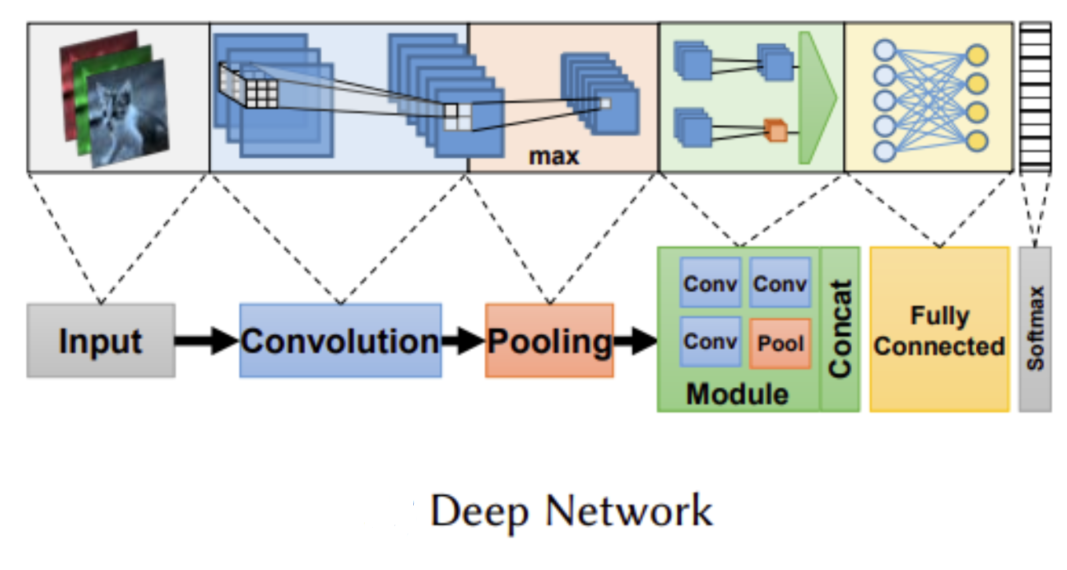
\includegraphics[scale=0.4]{Deep_1.PNG}
\end{center}
\end{frame}

\begin{frame}{Lý thuyết cơ sở}
\textbf{Nơ-ron}: \pause
\begin{enumerate}[-]
	\item Mô phỏng theo não người;
	\item Sử dụng hàm kích hoạt.
\end{enumerate}

\begin{center}
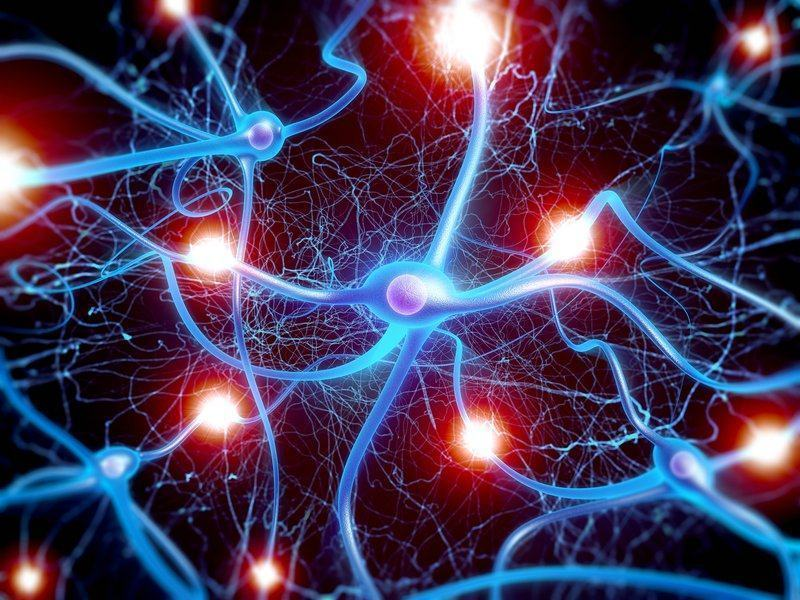
\includegraphics[scale=0.3]{neuron.jpg}
\end{center}
\end{frame}



\begin{frame}{Lý thuyết cơ sở}
\textbf{Mạng Nơ-ron}: 
\begin{center}
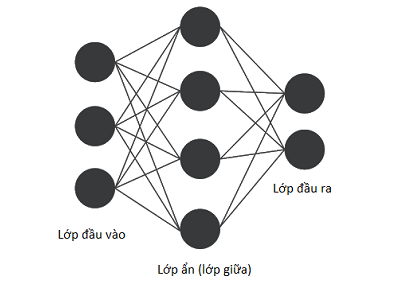
\includegraphics[scale=0.6]{ANN.png}
\end{center}
\end{frame}

\begin{frame}{Lý thuyết cơ sở}
\textbf{Các yếu tố trong huấn luyện mô hình Mạng nơ-ron}: \pause
\begin{enumerate}[-]
	\item Dữ liệu: \pause
	\begin{enumerate}[+]
		\item Dữ liệu lớn (Bigdata):
		\begin{enumerate}[i.]
			\item Dung lượng;
			\item Tính đa dạng;
			\item Vận tốc;
			\item Tính xác thực.\pause
		\end{enumerate}
	\end{enumerate}
	\item Mô hình;\pause
	\item Hàm mục tiêu;\pause
	\item Thuật toán tối ưu.
\end{enumerate}
\end{frame}

%%====
\begin{frame}{Kiến trúc máy tính song song}
\begin{center}
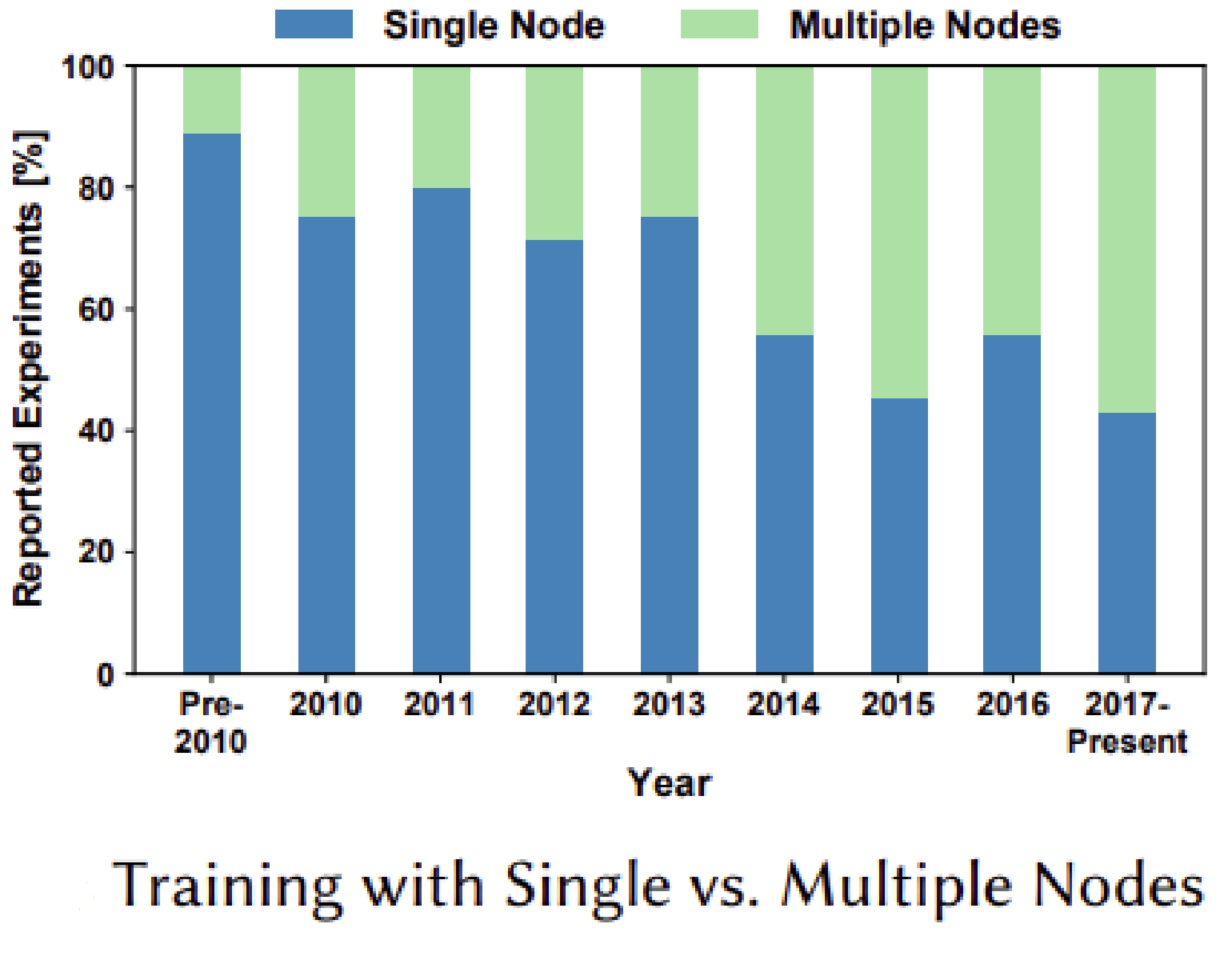
\includegraphics[scale=0.35]{KTSS1.PNG}
\end{center}
\end{frame}


\begin{frame}{Kiến trúc máy tính song song}
\textbf{Máy tính song song đơn (Single-machine Parallelism)}\pause
\begin{enumerate}[-]
	\item Đa tiến trình (multiple processes);
	\item Đa luồng (multiple threads);
	\item Kết hợp cả hai.
\end{enumerate}
\end{frame}

\begin{frame}{Kiến trúc máy tính song song}
\textbf{Đa máy tính song song (multi-machine Parallelism))}\\ \pause
Các chỉ số quan trọng nhất cho mạng kết nối là:
\begin{enumerate}[-]
		\item Độ trễ;
		\item Băng thông;
		\item Tỉ lệ truyền tin (Message-Rate)
\end{enumerate}
\end{frame}


\begin{frame}{Kiến trúc máy tính song song}
\begin{center}
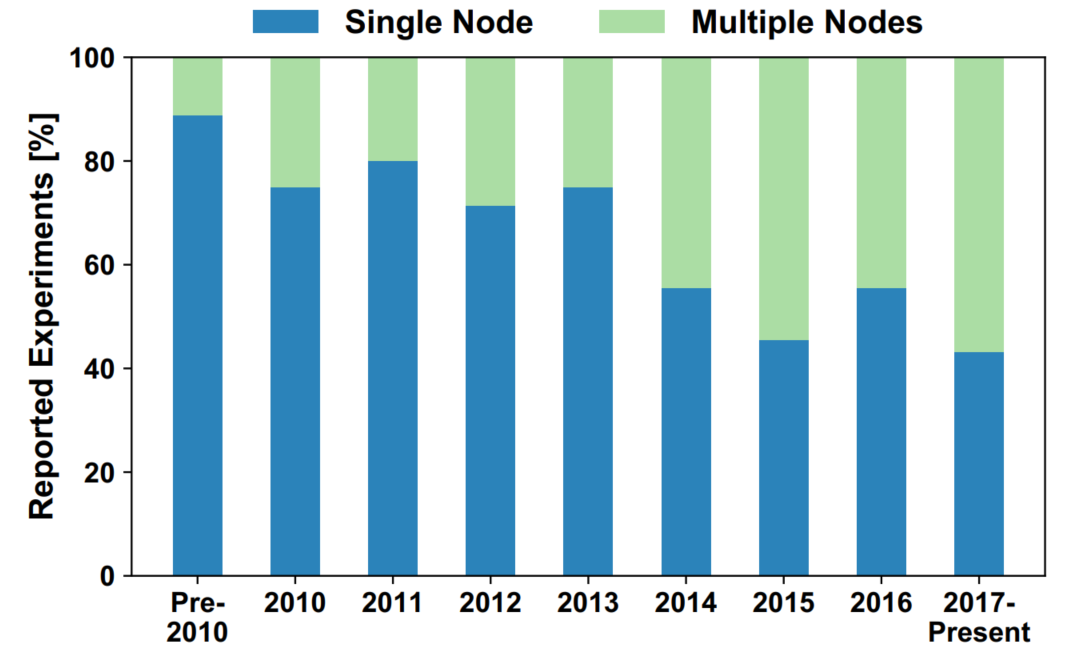
\includegraphics[scale=0.4]{multiNode.PNG}
\end{center}
\end{frame}

\begin{frame}{Kiến trúc máy tính song song}
\begin{center}
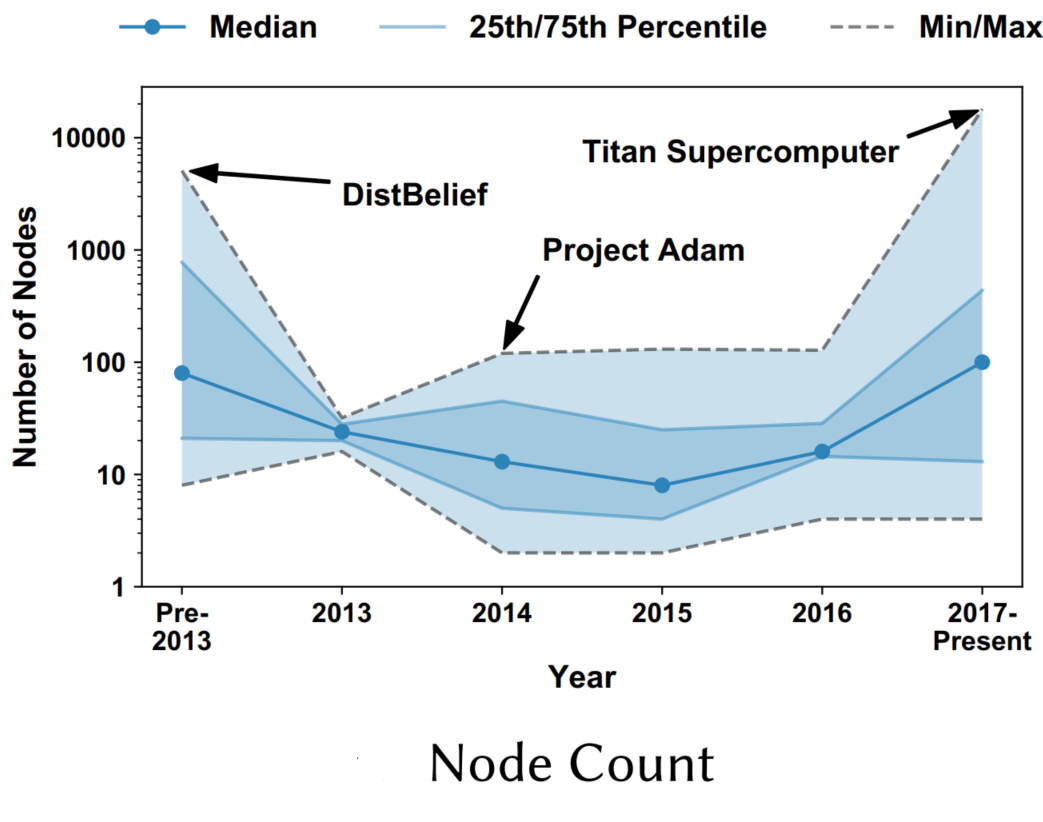
\includegraphics[scale=0.4]{multiNode2.PNG}
\end{center}
\end{frame}

\begin{frame}{Kiến trúc máy tính song song}
Ngoài ra, kiến trúc song song còn có:\\

\begin{enumerate}[-]
	\item Lập trình song song (Parallel Programming);
	\item Thuật toán song song (Parallel Algorithms);
\end{enumerate}
\end{frame}

\begin{frame}
\begin{center}
\Large Phần 2: Hệ thống học sâu phân tán
\end{center}
\end{frame}

\begin{frame}{ Hệ thống học sâu phân tán}
\textbf{Hệ thống học sâu phân tán (Distributed Deep Learning Systems - DDLS)} \pause
 là hệ thống đào tạo các mô hình mạng nơ-ron bằng cách sử dụng tài nguyên phân tán của một cộng đồng.
\end{frame}

\begin{frame}{ Hệ thống học sâu phân tán}
\textbf{Những vấn đề khi phát triển một hệ thống học sâu phân tán}: \pause
\begin{enumerate}[i]
	\item Tính nhất quán;\pause
	\item Khả năng chịu lỗi;\pause
	\item Khả năng giao tiếp;\pause
	\item Quản lý tài nguyên;\pause
	\item Mô hình lập trình.
\end{enumerate}
\end{frame}


\begin{frame}{ Hệ thống học sâu phân tán}
\textbf{Các chiến lược song song}: 
\begin{enumerate}[i]
	\item Song song dữ liệu (Data Parallelism);
	\item Song song mô hình (Model Parallelism);
	\item Kỹ thuật đường ống (Pipelining);
\end{enumerate}
\end{frame}

\begin{frame}{Hệ thống học sâu phân tán}
\begin{center}
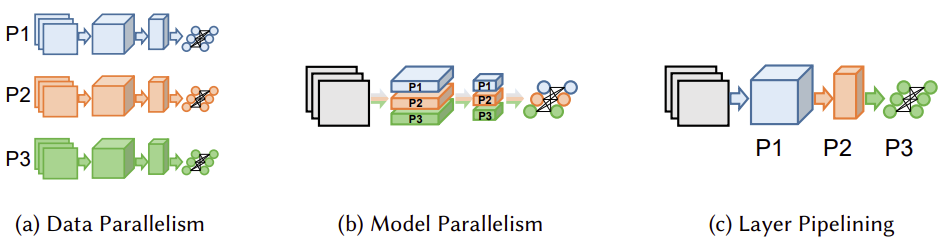
\includegraphics[scale=0.55]{parallel_1.PNG}
\end{center}
\end{frame}

\begin{frame}{Hệ thống học sâu phân tán}
\textbf{Song song dữ liệu: } \pause
\begin{enumerate}[i]
	\item Chia dữ liệu thành một số phân vùng, với số phân vùng bằng số lượng nút tính toán.
	\item Mỗi nút tính toán đóng vai trò như một công nhân sở hữu một phân vùng độc lập và mỗi công nhân thực hiện tính toán trên phân vùng của chính họ.
\end{enumerate}
\end{frame}

\begin{frame}{Hệ thống học sâu phân tán}
\textbf{Song song dữ liệu } \\
Cách tiếp cận:\\
\begin{enumerate}[i]
	\item Máy chủ tham số không đồng bộ (Async Parameter Server);
	\item Kiến trúc đồng bộ hóa giảm tất cả (Sync Allreduce Architecture). 
\end{enumerate}
\end{frame}

\begin{frame}{Hệ thống học sâu phân tán}
\textbf{Song song dữ liệu } \\
Máy chủ tham số không đồng bộ:
\begin{center}
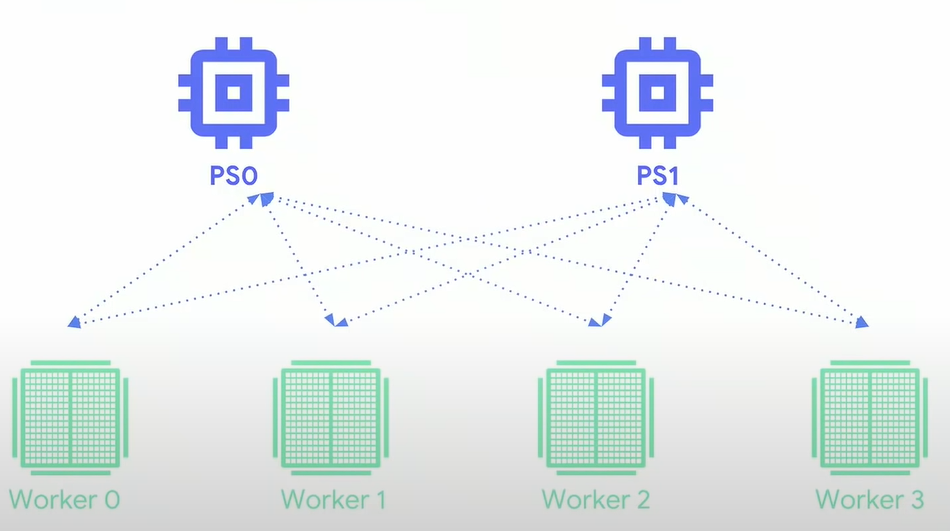
\includegraphics[scale=0.55]{Async.PNG}
\end{center}
\end{frame}


\begin{frame}{Hệ thống học sâu phân tán}
\textbf{Song song dữ liệu } \\
Kiến trúc đồng bộ hóa giảm tất cả:
\begin{center}
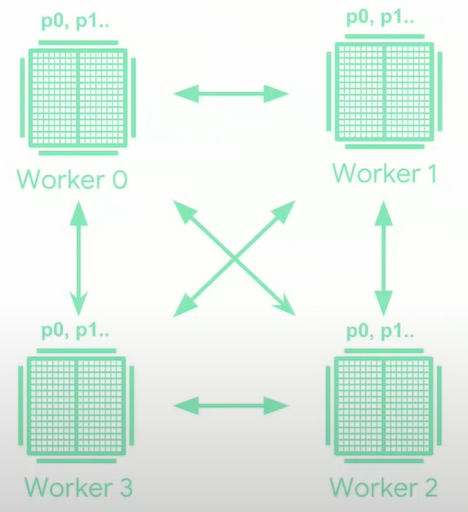
\includegraphics[scale=0.55]{sync.PNG}
\end{center}
\end{frame}


\begin{frame}{Hệ thống học sâu phân tán}
\textbf{Song song mô hình } \\
Thay vì phân vùng dữ liệu như song song dữ liệu, chúng tôi cố gắng phân vùng chính mô hình học sâu để phân phối khối lượng công việc cho nhiều nút (công nhân) tính toán.
\end{frame}

\begin{frame}{Hệ thống học sâu phân tán}
\textbf{Kỹ thuật đường ống } \\
Trong học sâu, pipelining có thể đề cập đến các phép tính chồng chéo, tức là giữa lớp này và lớp tiếp theo; hoặc phân vùng DNN theo độ sâu, gán các lớp cho các bộ xử lý cụ thể.
\end{frame}

\begin{frame}{Một số thuật toán tối ưu hóa phân tán}
2 quy trình tối ưu hóa phân tán quy mô lớn:\\
\begin{enumerate}[i]
	\item Downpour SGD;
	\item Sandblaster L-BFGS.
\end{enumerate}
\end{frame}

\begin{frame}{Một số thuật toán tối ưu hóa phân tán}
\textbf{Downpour SGD}:\\ \pause
\begin{enumerate}[i]
	\item Khắc phục hạn chế của SGD;\pause
	\item Cách tiếp cận cơ bản:\pause
	\begin{enumerate}[-]
		\item Chia dữ liệu huấn luyện thành một số tập con;\pause
		\item Chạy một bản sao của mô hình trên các tập con đó;\pause
	\end{enumerate}
\end{enumerate}
\end{frame}

\begin{frame}{Một số thuật toán tối ưu hóa phân tán}
\textbf{Sandblaster L-BFGS:} \\ \pause
\begin{enumerate}[-]
	\item Phương pháp lô (L-BFGS )hoạt động tốt trên mạng học sâu nhỏ; 
	\item Sandblaster giúp cải thiện điều đó;\pause
	\item Ý tưởng: lưu trữ và thao tác với tham số phân tán; 
\end{enumerate}
\end{frame}

\begin{frame}
\begin{center}

	\Large TensorFlow

\end{center}

\end{frame}

\begin{frame}

\Large Phần III: Một số kết quả

\end{frame}

\begin{frame}{Kết quả nghiên cứu tại Google Inc}
\begin{enumerate}[-]
	\item Mục đích:  đánh giá các thuật toán tối ưu hóa của họ bằng cách áp dụng chúng vào các mô hình đào tạo cho hai vấn đề học sâu khác nhau: nhận dạng đối tượng trong ảnh tĩnh và xử lý âm thanh để nhận dạng giọng nói; \pause
		\item Nhận dạng giọng nói: phân loại trạng thái âm thanh: \pause		        	\begin{enumerate}[+]
		\item Sử dụng mô hình học sâu 5 lớp, trong đó:
		\begin{enumerate}[o]
			\item Lớp ẩn: 2560 nút;
			\item Lớp đầu ra: 8192 nút;
		\end{enumerate}
		\item 42 triệu tham số;
		\item 1,1 tỷ bản ghi. \pause
	\end{enumerate}
	\item Xử lý ảnh: \pause
	\begin{enumerate}[+]
		\item 16 triệu ảnh;
		\item kích thước mỗi ảnh: 100x100 pixel;
		\item 3 giai đoạn: lọc, gộp và chuẩn hóa tương phản cục bộ;
	\end{enumerate}
\end{enumerate}

\end{frame}

\begin{frame}{Kết quả nghiên cứu tại Google Inc}
\begin{enumerate}[-]
	\item Mô hình gọng nói: \pause
Chạy trên 8 máy, có tốc độ tính toán \textbf{ nhanh hơn 2,2 lần} so với sử dụng một máy duy nhất. \pause
	\item Mô hình xử lý ảnh: 
Tốc độ nhanh hơn 12 lần khi sử dụng 81 máy.
\end{enumerate}
\end{frame}

\begin{frame}{Kết quả nghiên cứu tại Google Inc}
\begin{center}
	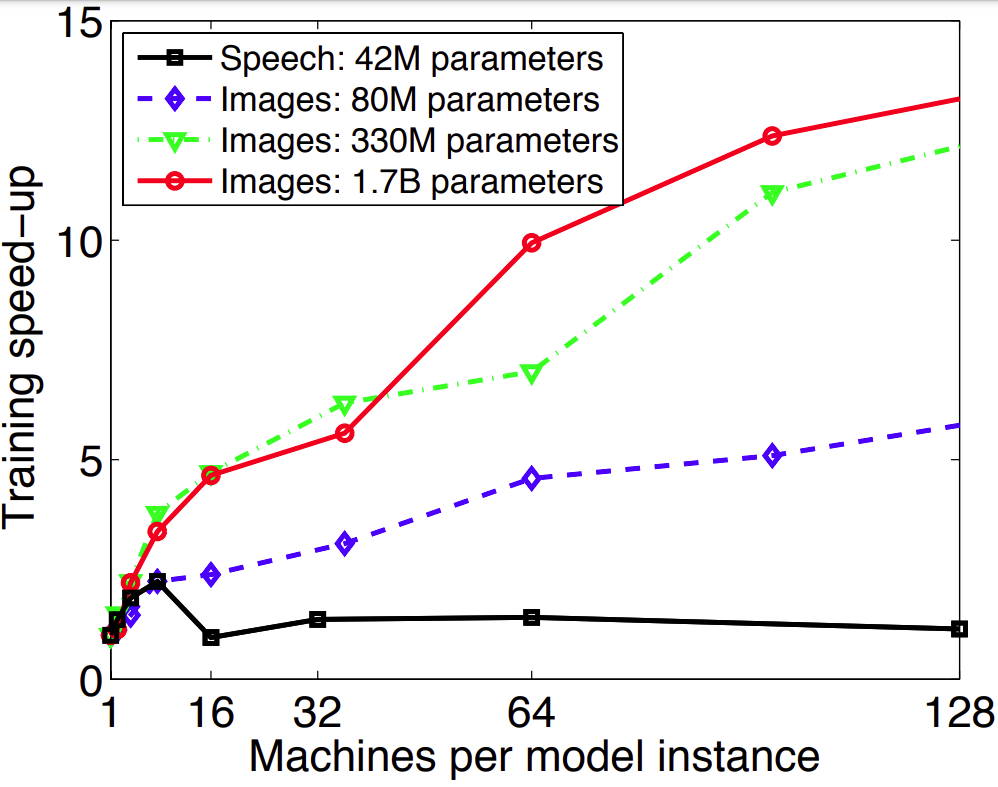
\includegraphics[scale=0.45]{GG_1.PNG}
\end{center}
\end{frame}

\begin{frame}{Kết quả nghiên cứu tại Google Inc}
\begin{center}
	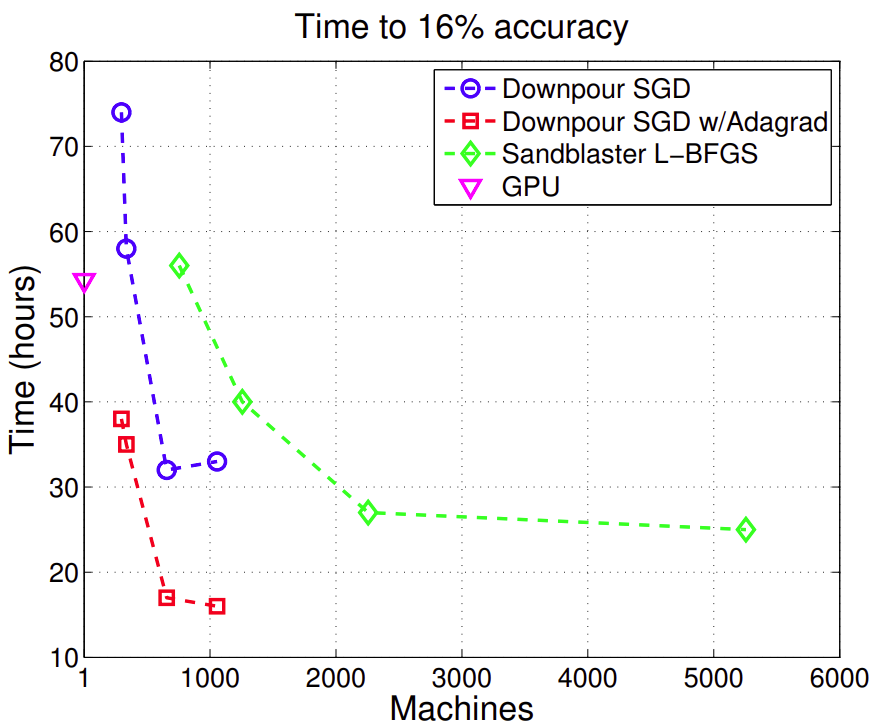
\includegraphics[scale=0.45]{GG_4.PNG}
\end{center}
\end{frame}

\begin{frame}{Kết quả nghiên cứu tại Google Inc}
\begin{center}
	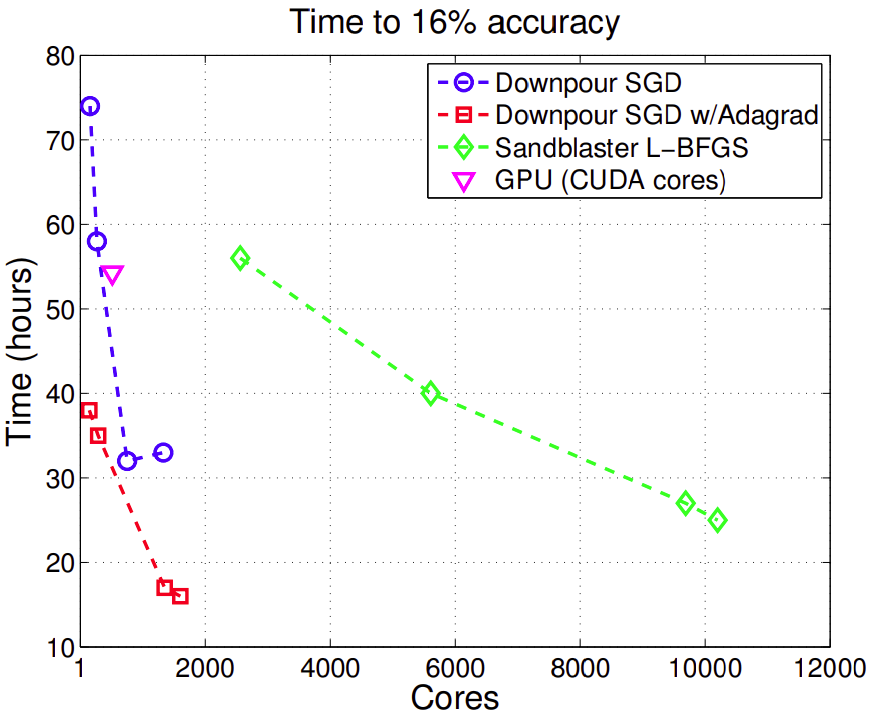
\includegraphics[scale=0.45]{GG_5.PNG}
\end{center}
\end{frame}

\begin{frame}{Kết quả nghiên cứu tại MIT}
\begin{enumerate}[-]
	\item Mục đích: Dự báo lượng mưa; \pause
	\item Triển khai trong TensorFlow 1.12 bằng cách sử dụng API Keras. Mạng này có 17.395.992 tham số có thể huấn luyện. \\\pause
	\item Chạy bộ dữ liệu đã có trên 1 GPU GK210, thu được: 	
	
	
\begin{tabular}{|c|c|c|c|c|}
\hline
        & \textbf{\begin{tabular}[c]{@{}c@{}}Số lượng ảnh\\ đào tạo\end{tabular}} & \multicolumn{1}{l|}{\textbf{\begin{tabular}[c]{@{}l@{}}Số lượng ảnh\\ kiểm tra\end{tabular}}} & \textbf{Epochs} & \textbf{\begin{tabular}[c]{@{}c@{}}Thời gian \\ đào tạo (giờ)\end{tabular}} \\ \hline
Bộ DL 1 & 17,833                                                                  & 10,052                                                                                        & 100             & 23.219                                                                      \\ \hline
Bộ DL 2 & 45,897                                                                  & 10,052                                                                                        & 100             & 59.136                                                                      \\ \hline
\end{tabular}
\end{enumerate}
\end{frame}

\begin{frame}{Kết quả nghiên cứu tại MIT}
\begin{enumerate}[-]
	\item TensorFlow / Keras và sử dụng framework Horovod;
	\item 32 nút với 4 thiết bị GK210 trên mỗi nút, trong tổng số 128 thiết bị GPU.
\end{enumerate}
\end{frame}

\begin{frame}{Kết quả nghiên cứu tại MIT}
\begin{center}
	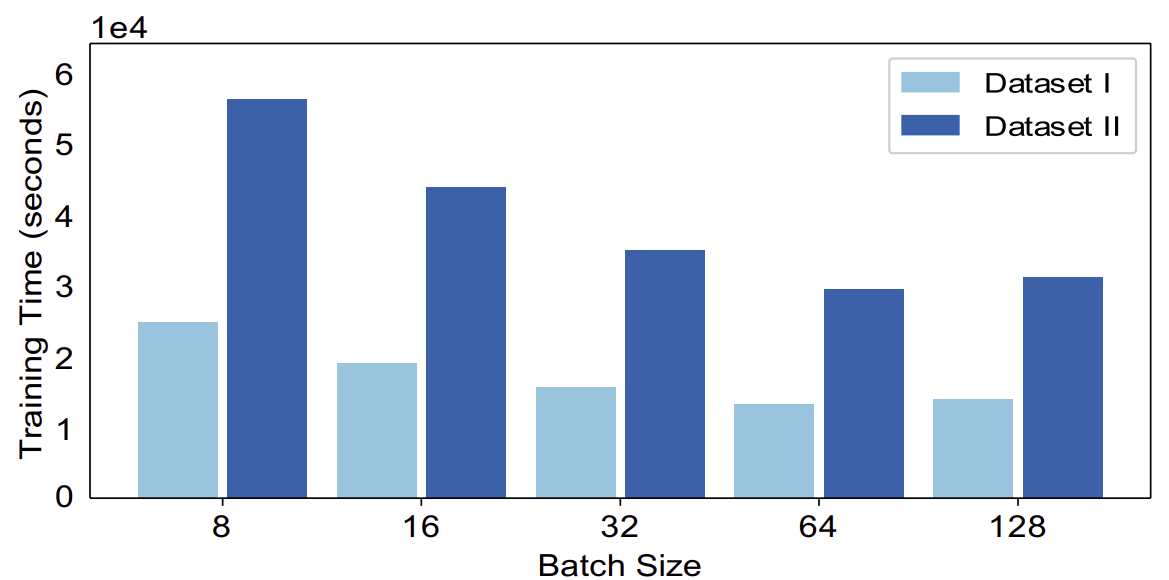
\includegraphics[scale=0.42]{MIT_1.PNG}
\end{center}
\end{frame}

\begin{frame}{Kết quả nghiên cứu tại MIT}
\begin{center}
	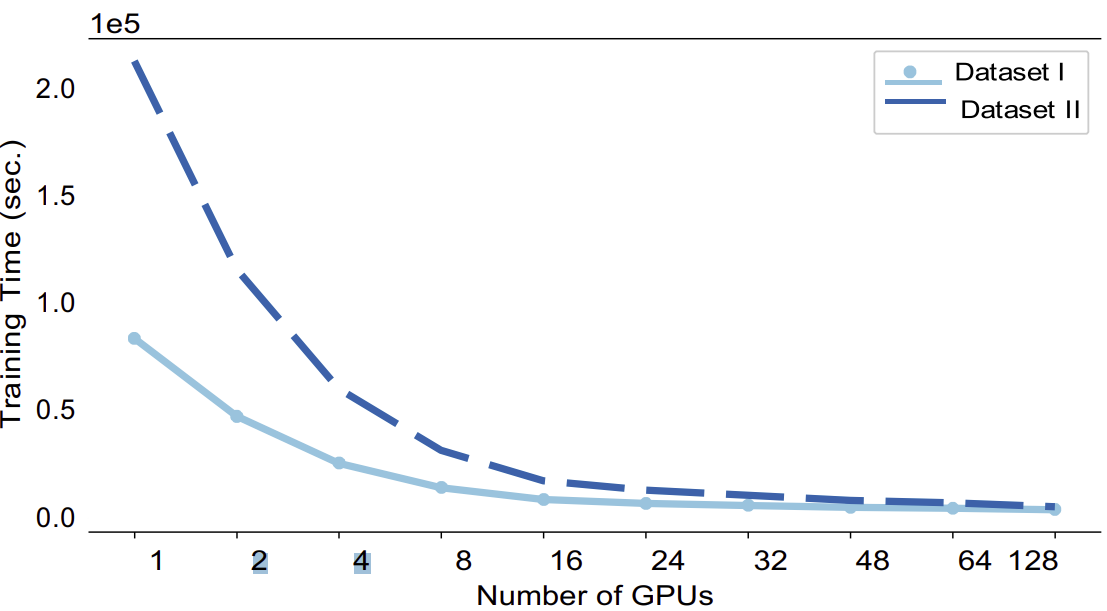
\includegraphics[scale=0.42]{MIT_2.PNG}
\end{center}
\end{frame}


\begin{frame}{Kết quả nghiên cứu tại MIT}
\begin{center}
	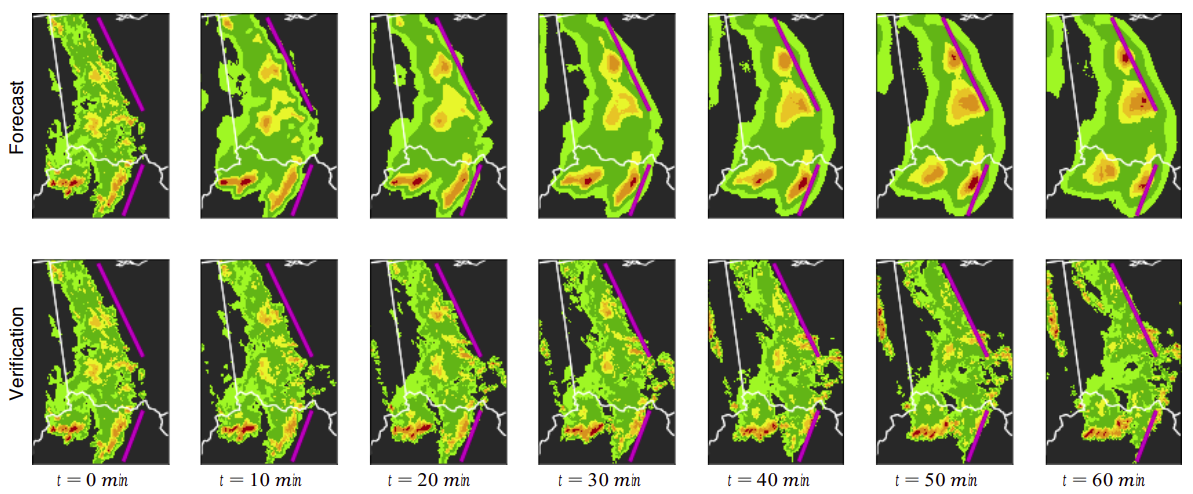
\includegraphics[scale=0.42]{MIT_4.PNG}
\end{center}
\end{frame}

\begin{frame}{Kết quả chương trình Demo}
\begin{enumerate}[-]
	\item Thực hiện trên Ubuntu với thư viên phân tán của TensorFlow; \pause
	\item Thực hiện trên 1 thiết bị laptop và mở nhiều cổng;
	\item Các cổng thông nhau thông qua giao thức TCP/IP.
\end{enumerate}
\end{frame}

\begin{frame}
\begin{center}
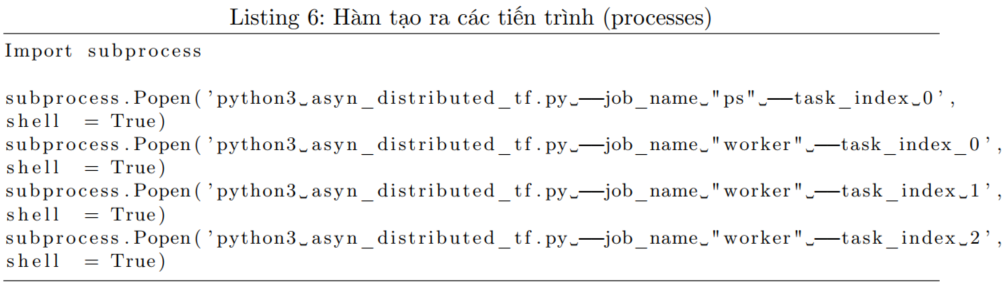
\includegraphics[scale=0.52]{CODE1.PNG}
\end{center}
\end{frame}

\begin{frame}
\begin{center}
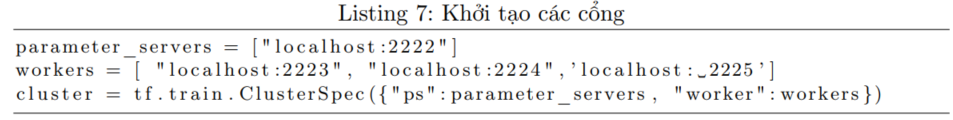
\includegraphics[scale=0.52]{CODE2.PNG}
\end{center}
\end{frame}

\begin{frame}
\begin{center}
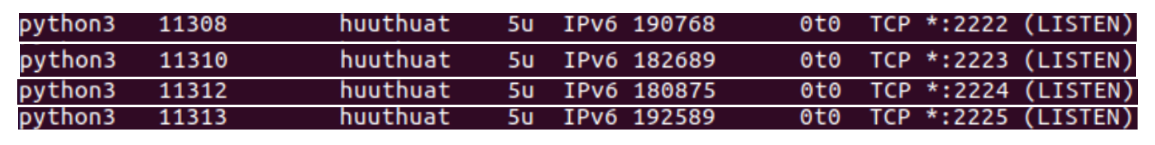
\includegraphics[scale=0.45]{IP.PNG}
\end{center}
\end{frame}


\begin{frame}
\begin{center}
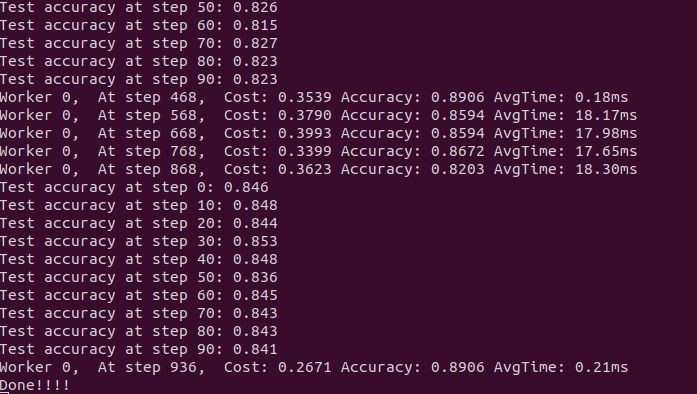
\includegraphics[scale=0.45]{Dis_1.PNG}
\end{center}
\end{frame}


\begin{frame}
\begin{center}
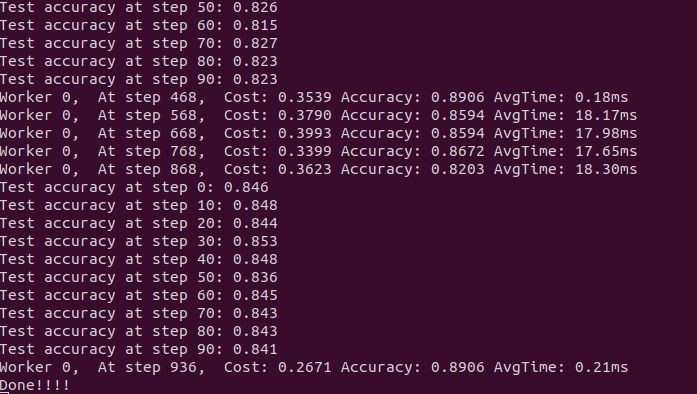
\includegraphics[scale=0.45]{Dis_1.PNG}
\end{center}
\end{frame}

\begin{frame}
\begin{center}

\includegraphics[scale=0.4]{thanks.png}
\end{center}
\end{frame}








\end{footnotesize}
\end{document}